\section{Solution}
\label{sec: Methodology}
\par \textit{"Lina, your colleague and friend, did not appear today in class and your teacher knows that she will not come to school anymore, but does not know why. Although she sees your messages, does not answer them, she just sends an enigmatic image that appears to be on your desk. What could that mean?"}
\par With the first paragraph as premise, LINA is a mobile Augmented Reality videogame inserted in the D.O.T. - Die Offene Tür project \cite{dot_project_website_2017}, aiming towards "improving social connectedness through digital experiences". LINA aims to create an immersive experience, where the players take on the role of students in a class and engage with each other, guided by the game. This allows the players to socially connect themselves free of prejudice, acting as a field-levelling tool by providing them with an isolated fictional environment and by portraying (and socializing as those) fictional characters. Having begun focusing on the COPMI - Children of Parents with Mental Illness - the game has now broaden its target group to all children in the middle school ages (10-12 year olds) as they can also benefit from the fictional space that the game creates, as prejudice is not exclusive to children with special needs.

\begin{figure}
	\centering
	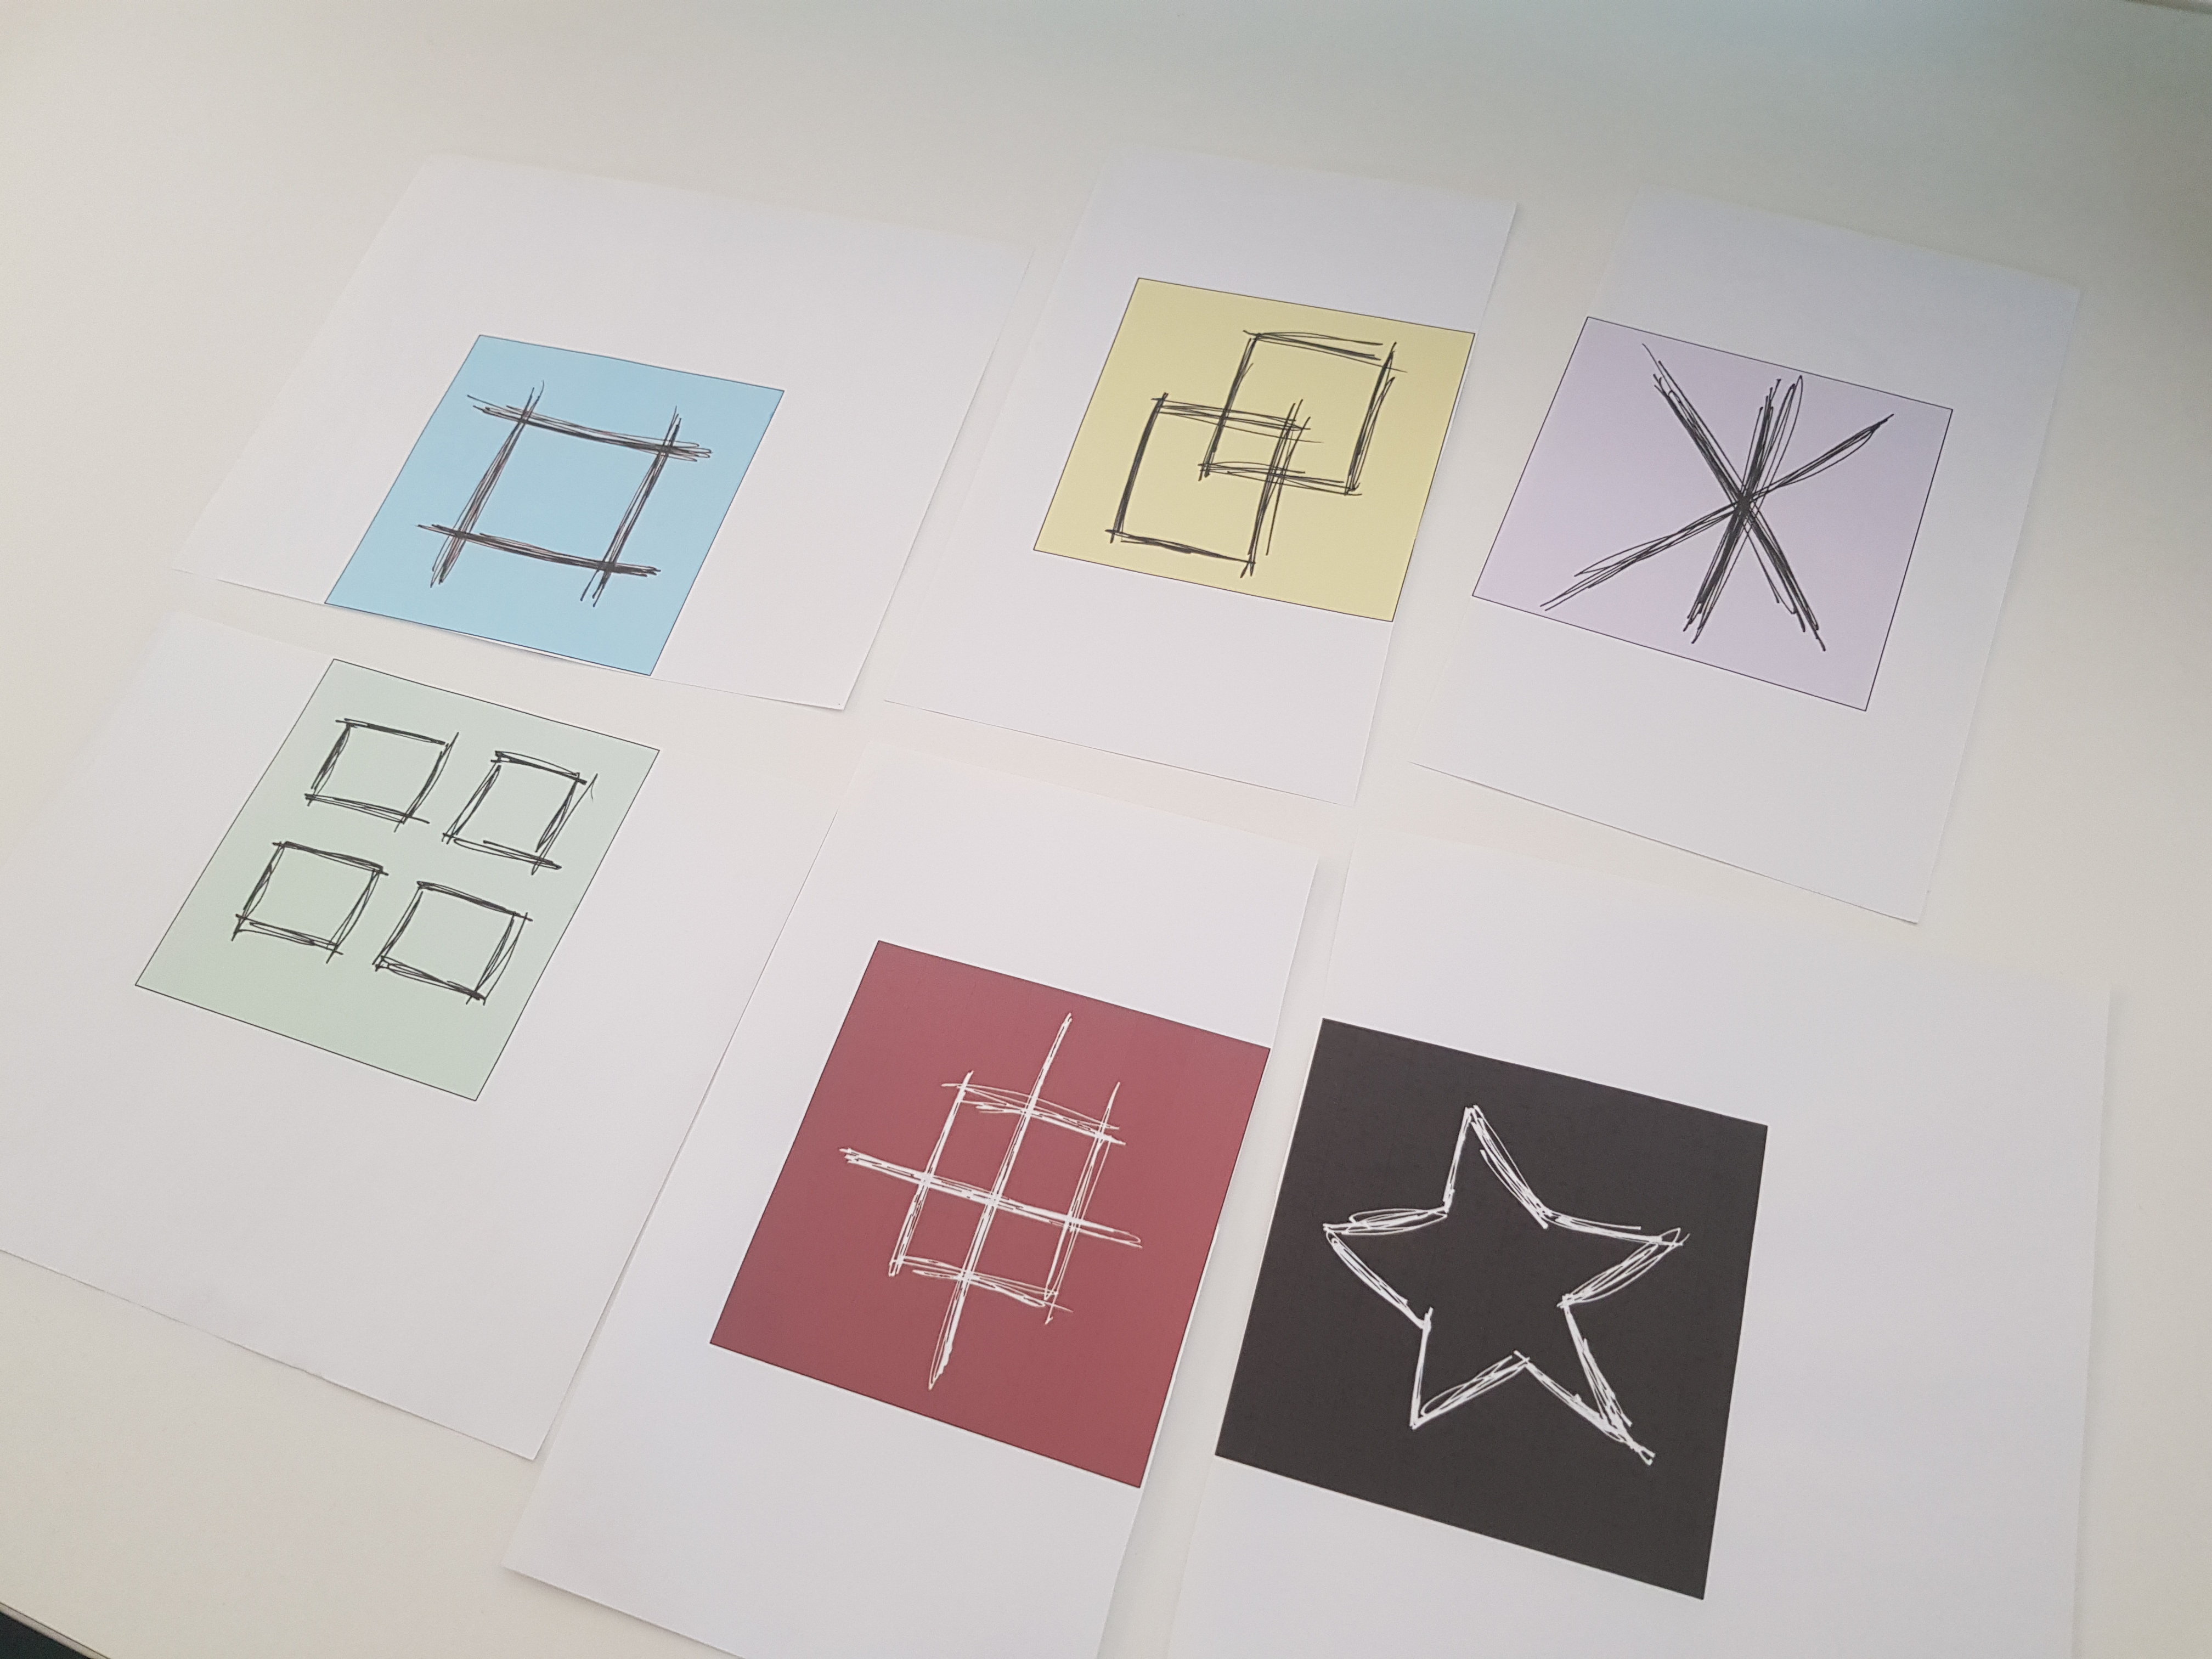
\includegraphics[scale = 0.05]{newIcons.jpg}
	\caption{The markers that are to be recognized and overlayed through Augmented Reality.}
	\label{fig:icons}
\end{figure}



\subsection{Concept} The basic concept of LINA is the search for a clue through the use of overlayed augmented reality over a marker. When scanning an image [Fig. \ref{fig:icons}] with the device's camera, an overlayed clue (usually an object that the player can interact with) is revealed, usually describing an important event involving Lina, followed with instructions to search for another image.
\par After the player completing 1 or 2 "stages", they must find another player - or group of players, henceforth designated as element - and solve a challenge presented to them. These challenges could be answering questions about the parts of story that only the other player knows about (which forces them into socializing when sharing their parts of the story), or having both elements perform a task together, for example simultaneously scanning a set of markers. This way the game creates an interesting way of socializing while at the same time exploring a narrative that relates to social isolation. This gives us the four ``positive factors" mentioned in Contact Theory:
\begin{itemize}
	\item Equal status between groups - All children will have the same importance in the game, all have important information that need to be shared among the others so that they can all advance in the narrative;
	\item Common goals - The shared goal is to overcome challenges and finish the game and find what happened to Lina.
	\item Inter-group cooperation - Only by sharing the information, or completing challenges together can they advance in the narrative, so there must be cooperation among themselves.
	\item Support of authorities, law or custom - The teacher, being the authority figure in the classroom, has given the explicit approval and is even directly involved in the game.
\end{itemize}
These ``stages" are not the same for all players: different players would get different stages so that they would get different pieces of the puzzle.
\par As the complexity of the game increases due to the elements scaling, multiple approaches have been discussed regarding the game's structure. Originally, each student started on his own and slowly paired up with his colleagues until the whole group searched for the final clue as one, like a perfect binary tree, with each node being an element: a leaf node representing a student, a non-leaf node representing a pairing and the root node the whole class. This structure would only work if the number of students in the class was a power of two, or else a student would have to either play alone while others were already paired, or skip stages to pair with a larger group, which would be unbalanced. Plus, the number of stages could be inappropriate to accommodate the number of students in class. 
\par Then it was considered to split the class in smaller groups of students, with each group playing LINA separately instead of being a single class, but that would defeat the purpose of pairing the children with someone that they get along with, plus it doesn't address the issue with the previous strategy.
\par Then it was concluded that instead of trying to make the number of stages according to the number of players, it should be the opposite: establish a fixed number of stages and split the class accordingly into groups of a pre-established size. For example, if a certain challenge needs elements of 4 or 5 persons then in a class of 9 it would split into [4,5], in a class of 18: [4,4,5,5], in a class of 23: [4,5,5,5,4]. Then at the end of the challenge the next elements are reshuffled (or perhaps the system could know which colleagues the player hasn't been paired with - needs further discussion) However it is necessary to first know how many stages LINA has before starting to split the class into groups, and then make the challenges flexible to accommodate groups of N or N+1.


\subsection{Structure, Challenges \& Story}
\par Presently, it has been discussed splitting LINA in sessions (or "episodes"): 5-10 minutes of recap in the beginning; 30-35 minutes of gameplay, where the children play some stages, initially by themselves, later in groups; and 10-15 minutes of discussion afterwards. 
\par A stage is the basic gameplay unit, similar to a level. There are 5 core stage archetypes in LINA:
\begin{enumerate}
	\item A roleplay-style stage, where the players are instructed to say something, or act in a certain way;
	\item A narrative-related stage, where the player only needs to pay attention to the narration or to the text presented to him in his screen;
	\item A simple find-the-marker stage where the player is tasked to find a marker, then has to interact with an object and finally gets a piece of information that either develops Lina's character or his character. 
	\item A find-the-marker stage that differs from the previous archetype when the information or objects gathered in this stage is going to be useful in a cooperation stage later on.
	\item And a cooperation stage where the players need to work together to complete a challenge. This relates with Contact Theory, where each player has the same importance in working towards the common goal.
\end{enumerate}

\par So far there are 7 different stages in the game:
\begin{itemize}
	\item Stage 1 - Registration and Initial Briefing: 
	\par An example of the first archetype, in this stage the students and the teacher engage in a role-playing scene where the teacher is making the presence list, with each student answering his/her (character's) name, and by failing to call Lina the class gets intrigued with her absence, moving on to the next stage.
	
	\item Stage 2 - \textit{Lina's Message}: 
	\par An example of the 2nd archetype, in this scene the player's character wonders how strange it is that Lina did not show up for class. He thinks to himself whether he should text Lina. After texting Lina asking what happened to her, she only answers back with a mysterious image. "What does that mean?" the player's character wonders. This prompts the player to search for this picture and thus setting up the premise for the first mission. As each player is going to search for a different image, the received image is going to be different for each player, making the number of different markers varying with the number of students in class.
	
	\item Stage 3 - \textit{Tutorial}: 
	\par \textit{Tutorial} is an example of the 3rd archetype, the first mission and entry point for the player into the proper game. After receiving the mysterious image from Lina's message, the player needs to find what it means. The markers will be placed directly on the player's desk, just to introduce them to the core mechanics of the game, like scanning and tapping the marker.
	
	\item Stage 4 - \textit{The Party and The Note}/\textit{The Picture On The Wall}: 
	\par This stage is another example of the 3rd archetype. In \textit{The Party and The Note} the player finds a crumpled-up paper that unravels a note that reveals that Lina didn't want to go to a colleague's birthday party. \par While one player is playing \textit{The Party and The Note}, another player is playing \textit{The Picture On The Wall}. In it he finds, upon scanning the marker, that art is Lina's best subject and that, when asked to draw someone that inspires her, she the drew the back of a hoodie.  \par \textit{The Picture On The Wall} was an idea from the original proof-of-concept where the students would have several drawings shown on a wall in real life, with a marker replacing Lina's drawing, prompting the students to scan the marker to see it the drawing, and make it as seamless as possible.
	
	\item Stage 5 - \textit{The Broken Screen}/\textit{The Broken Screen - Lina's PoV}: 
	\par Like Stage 4, \textit{The Broken Screen} and \textit{The Broken Screen - Lina's PoV} are two missions played in parallel by different players, that differ from the previous ones as they are setting up the cooperation stage that follows, falling under the 4th archetype. \par In \textit{The Broken Screen} the player finds a folder containing a letter from the teacher, Mr.Gordon, to the headmaster explaining how he found Lina and Ashley standing next to a broken computer. Lina first says that she and Ashley were the culprits but later she confesses to Mr.Gordon to have done it by herself.
	\par In \textit{The Broken Screen - Lina's PoV} the other player finds a note inside a backpack that reveals that Lina did not break the screen but it was in fact two older kids that bullied her into confessing the misdeed, and that Lina will correct things up, but did not say how.
	
	\item Stage 6 - \textit{Cooperative Question}: 
	\par When scanning the marker, the player finds an instruction telling to wait for the other player. When both players are at the marker they are asked to answer a question about the other player's part of \textit{The Broken Screen} story, which prompts the players into sharing their parts so they can answer the questions. When they correctly answer the question they unlock an instruction to find the next marker. This stage is an example of the 5th archetype.

    
	
	\item Stage 7 - \textit{Lina's Diary and Puzzle} - Archetypes 4 and 5:
	\par After unlocking the next marker in the challenge the players must find as a pair. When scanning the marker each player gets a different half of a page of Lina's diary. They are taken to a screen with four different images. The images are the same for both players, but their order differs. They are then instructed to tap on the images by the order they see on the other player's device. When they do so correctly both parts of the page unite to become a single page. One of the players is then asked to read Lina's diary to the other. This stage is a combination of archetypes 4 and 5 since there is a marker to be found but also a challenge after finding the marker, but does not make sense splitting into two different stages. 
	
	
\end{itemize}

\par It is necessary to reiterate that this project is still more than a proof-of-concept and that multiple approaches on how the game would be deployed have been considered, so the structure is subject to eventual changes. 
The first episode is an introduction, the next three the story development and the last episode concluding the story with the discovery that Lina has been acting strange due to her parents being affected with a mental illness.

\subsection{User Experience Design}

\begin{figure}
    \centering
    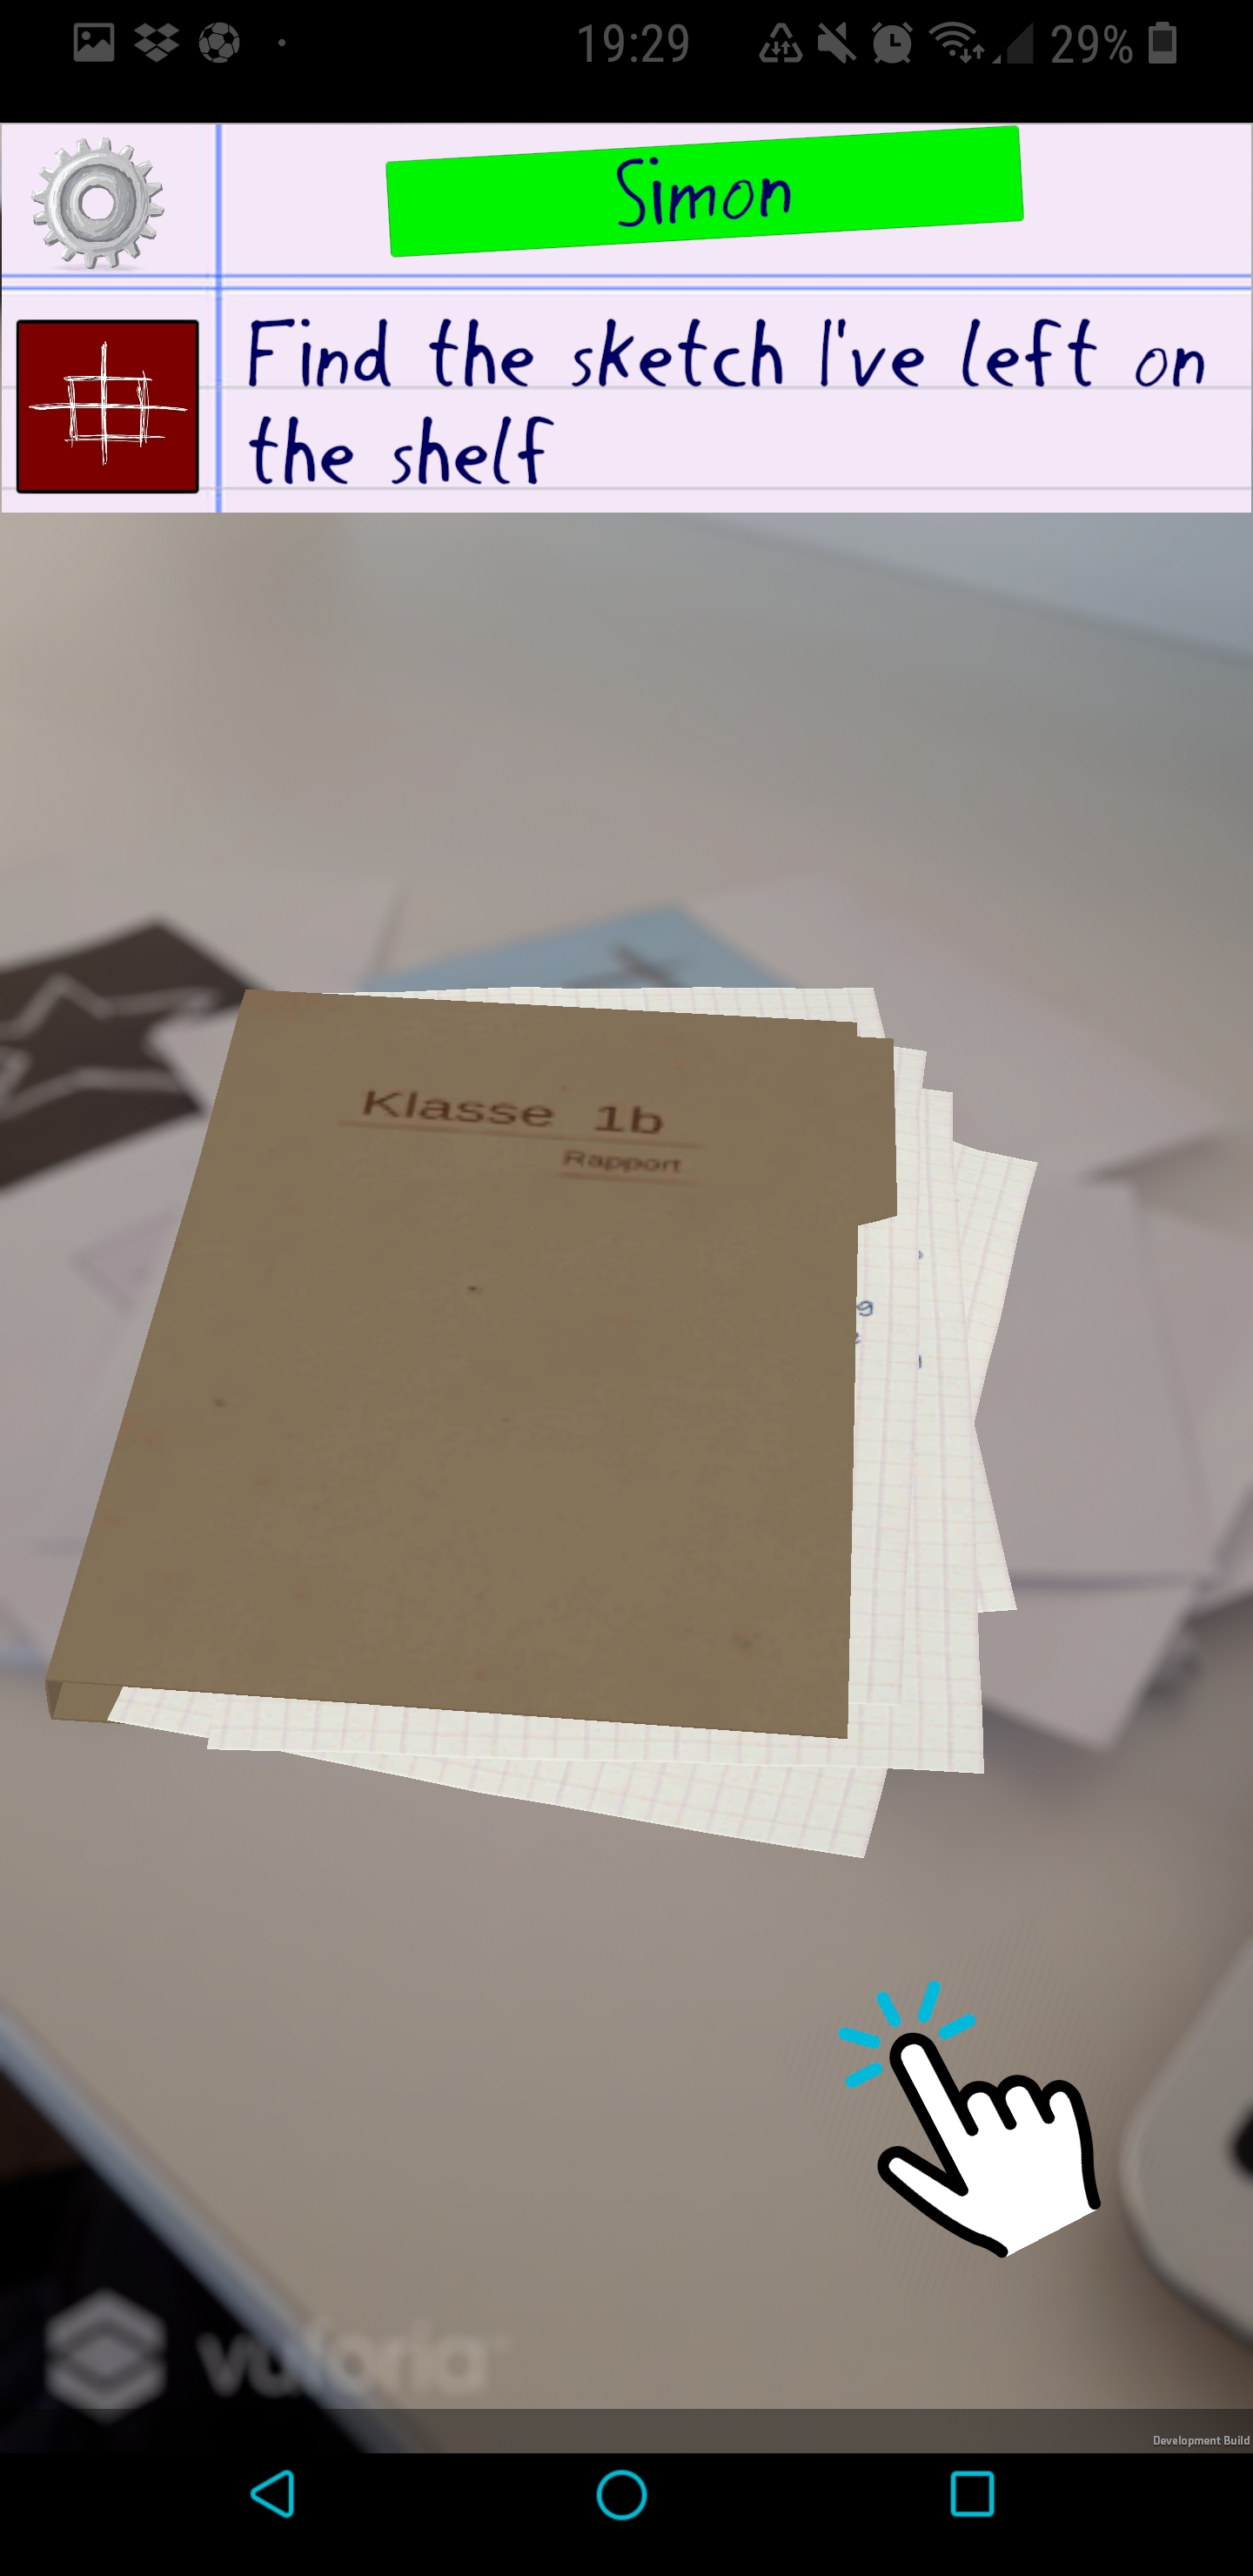
\includegraphics[scale = 0.07]{Screenshot_20190518-192941_LINA.jpg}
    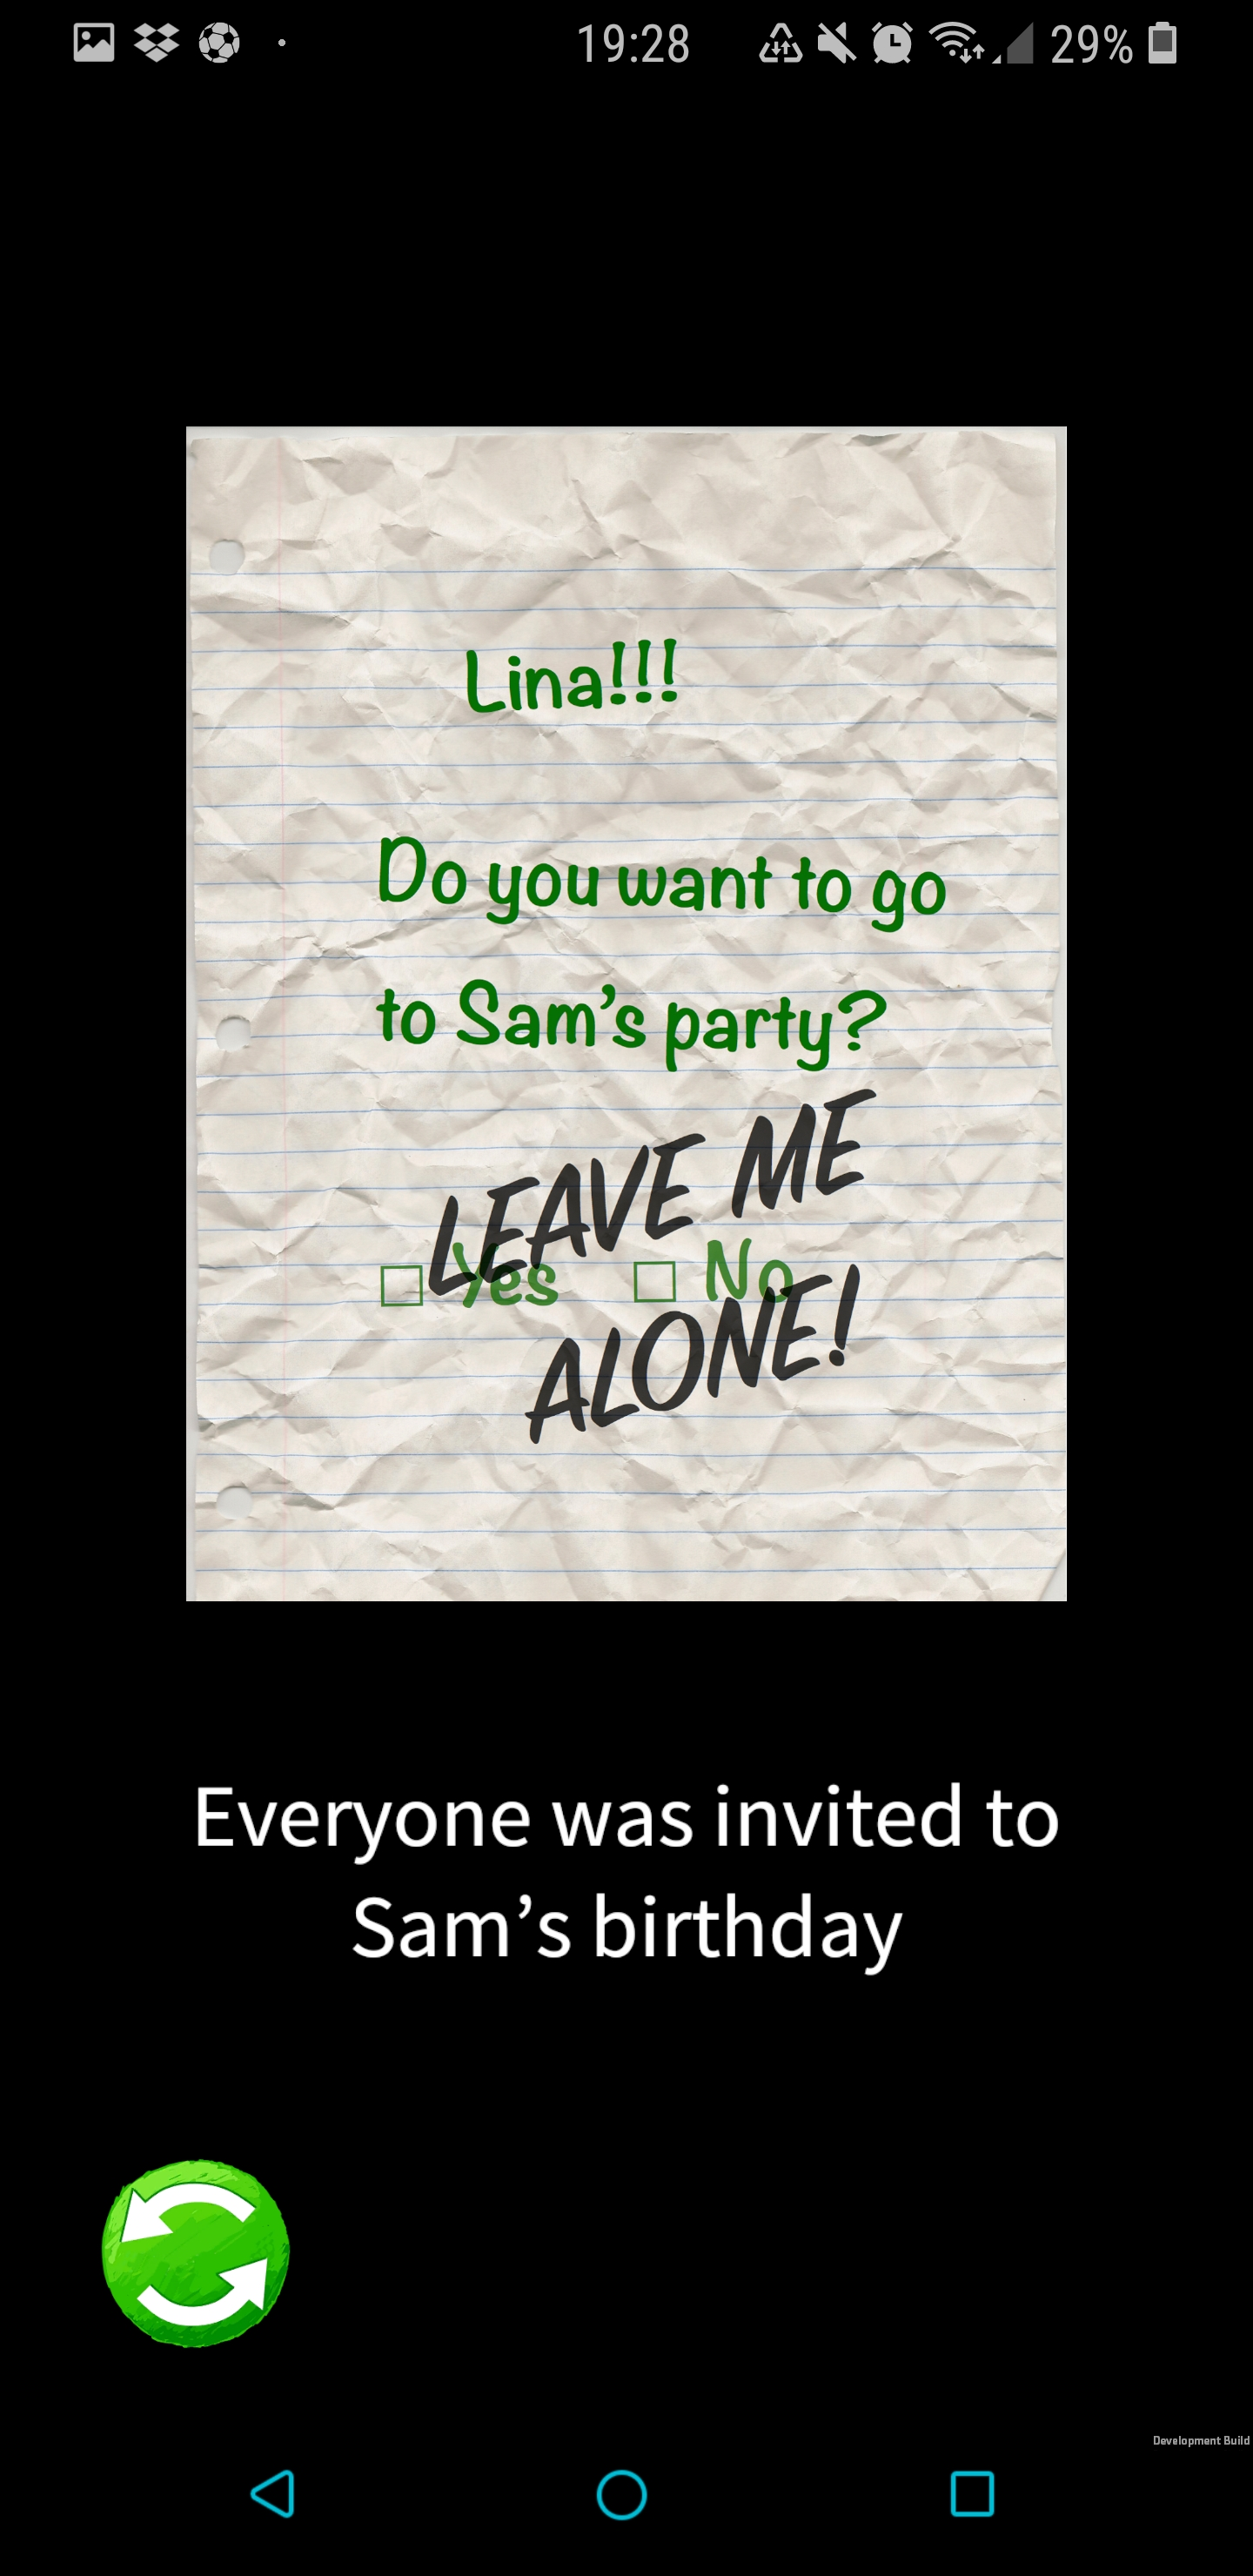
\includegraphics[scale = 0.07]{Screenshot_20190518-192847_LINA.jpg}
    \caption{These screenshots were taken from the second digital prototype: a) \textit{Exploration Mode}; b) \textit{View Mode}.}
    \label{fig:digital}
\end{figure}

\subsubsection{Usability}
\par In terms of usability, the game can be also divided in game modes: \textit{Exploration Mode}, \textit{View Mode}, and \textit{Interface Mode}. The player in each stage plays through one or more of these modes.
\par\textit{Exploration Mode} is the main scene in LINA, it is where the core mechanic of searching the world through imaging recovered live from the rear camera occurs. This was also the scene prone to more changes during the development. The recurring mechanic in a archetype 4 stage is: when the player scans a marker an augmented object appears, which the player needs to interact by tapping. Tapping that object usually unveils the real clue, and tapping on the clue usually triggers a narration and sends the player into \textit{View Mode}.
\par \textit{View Mode} is a screen where the players are shown an object relevant to the player. This was born out of the necessity of having a separate screen where the player could read an image containing text without having to keep the device scanning the marker. This screen also proves useful in presenting new objects that did not necessarily come from scanning a marker, for example, after the question challenge, when the new marker and instruction is unlocked.
\par \textit{Interface Mode} is any other scene where the player interacts with an interface, like when listening to its character narration or a in challenge. This usually follows the hand-script text on a notebook-style background, but not always: an example is the \textit{SMSApp} with its own style imitating a messaging application.

\subsubsection{Aesthetics}
\par In LINA there is a conscious effort to pass an immersive and atmospheric, almost cinematographic, feeling when playing the game. For that we made a number of decisions regarding the aesthetics: \textit{Exploration Mode} includes an atmospheric background music that accompanies the search for the markers, and sound effects when necessary. Also in "Exploration Mode", several post-processing filters like Grayscale, Sepia and Gaussian Blur were tested with the purpose of knowing the technical boundaries and what were the different cinematographic feelings conveyed. In particular, the Grayscale filter has been decided to be used in missions that are "flashbacks", being a typical visual effect used in media for that purpose; and the mixture of a blurred background and the sharp overlayed item provided a good effect aesthetically.
\par We also strive for realism with the markers and augmented reality clues, by trying to use realistic models. Pairing with the concept that art is Lina's best subject, the scribbled markers can become part of story, as if they were made by her, adding another layer of depth to the game. The design of the markers was changed in the middle of the development to fit the more realistic style [Fig.\ref{fig:icons}].
There is also a recurring art theme in the game: the hand-script on a notebook-style paper, as if the whole game was handwritten by Lina herself. This is further reinforced with an effort to have all interface images and buttons being drawings.
\par We also relied in established metaphors when designing the interface, not wanting it to be confusing and creating an obstacle that prevented the players from enjoying the experience: the "dented wheel" means settings, an arrow pointing right means "continue" and circular arrows mean "replay" (restarts the narration).

% #############################################################################

\subsection{Implementation}
The game was subject to several revision iterations, being developed first a low-fidelity prototype [Fig. \ref{fig:LFP}] from a supplied proof-of-concept document, then it was shown to experts and the playwright responsible for the narrative, iterated again, shown to the experts, and then developed a first version of the digital prototype, and then shown to the experts once more.
\par When designing the second prototype a design team was assembled, involving a playwright\cite{adam_barnard_2019} (tasked with designing the narrative) and a children psychologist, having weekly meetings regarding LINA and its design decisions. Due to time constraints it was not possible to have children testing the several prototype iterations, only the last one.

\begin{figure}
    \centering
    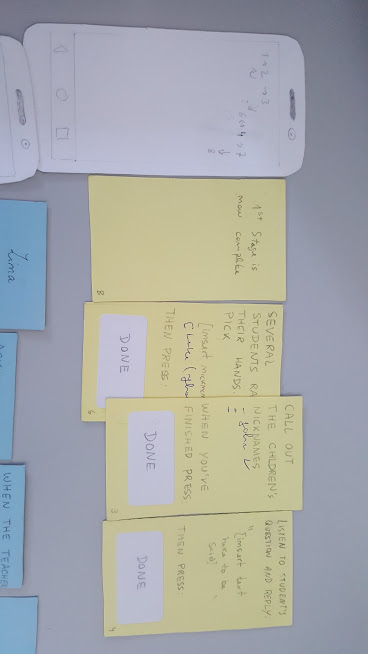
\includegraphics[scale = 0.3, angle = 90]{paper_proto1.jpg}
    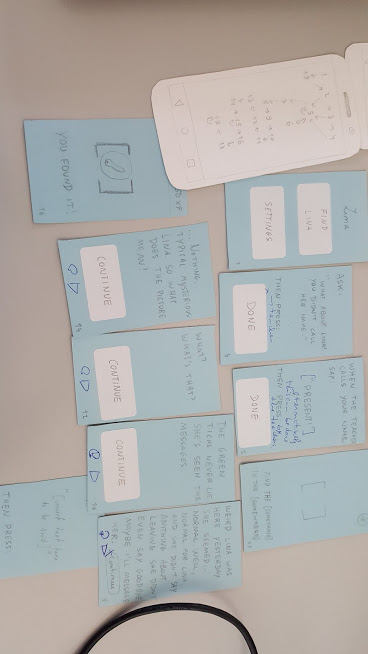
\includegraphics[scale = 0.3, angle = 90]{paper_proto2.jpg}
    \caption{Low-Fidelity Prototype of the teacher's and children's screen, respectively.}
    \label{fig:LFP}
\end{figure}

\subsubsection{Paper prototype} An initial low-fidelity paper prototype [Figs.\ref{fig:LFP}]was developed to conceptualize the interface and give some rough guidelines to fulfill the given script. A revision was made after presenting it to specialists where some suggestions regarding the presentation of some information texts and buttons.
\par The interface was chosen to be a simple area of text with some buttons on the bottom of the ``screen" (usually ``Back" and ``Next"), as to keep it simple, so that small children will not be distracted so easily, and to be intuitive, without ambiguities nor entropy. Blue and yellow colors seemed a very pleasant, non-intrusive and neutral background for the players and teacher, respectively.


\subsubsection{First digital prototype} The first digital prototype was made in the Unity3D Engine for its multi-platform support, and the Augmented Reality plug-ins that could be used to implement the scanning part. Initially, we thought that the markers could be QR codes to be scanned, however we decided to go directly for printed pictures instead, as the cost for implementation would be the same and there wasn't an advantage in starting with QR codes and changing to printed images later on.
\par For the Augmented Reality part we used \textit{Vuforia Augmented Reality SDK}, a plug-in that allows 2D or 3D ``markers" to be recognized and overlays an image or object in a position relative to the marker. The game uses a client-server approach to handle communication between the devices, as there must be a server app running as a game controller. This server also handles the synchronized communication used in the introduction, for example, where a dialogue scene must be coordinated between the teacher and his students. Contrary to the client apps, the server will be run in a computer.


\subsubsection{Second digital prototype} A second, and current, digital prototype [Fig.\ref{fig:digital}] was developed with the goal of presenting a minimal viable product for user testing. With this iteration we could experiment with the User Interface to see what would convey the feeling of the experience better - as it is supposed to have a realistic feeling, although a bit cartoon\textit{-ish}, due to Lina's drawings. Plus, some story was added and the cooperation parts were refined. 
\par For this prototype there was no need for a running server (as it was focused on the gameplay and the atmospheric feeling that was trying to be passed) so it was decided to make this version a local client where the user could choose between two "mock-up" players - Simon and Max - avoiding unnecessary complexity and the faults and could be derived from there. As the second prototype doesn't have a server and was just for showcasing purposes, the initial dialogue is skipped. Instead, there is an introduction video describing the initial exposition by the teacher.

% #############################################################################

\subsubsection{Changes Made for the Evaluation Workshop}

\par Some changes had to be made to the prototype for it to be properly played in the evaluation workshop. For instance, all text was translated to German. The note images that were written in English were left untouched, as was the audio narration, as there was not enough time to replace them for German translated ones and to be ready in time for the workshop.
